% Part   : Concepts
% Chapter: Scripts
% ------------------------------------------------------------
% $Id: scripts.tex 6207 2010-08-05 13:11:13Z al $
% ------------------------------------------------------------

\begin{description}
\item[framework:] trunk/Scripts/
\end{description}

\noindent Inside CentOS Artwork Repository, scripts are organized in
three groups: ``invocation scripts'', ``configuration scripts'' and
``function scripts''. Scripts are mainly used to help you automate and
standardize tasks. A graphical representation of how scripts are
organized inside CentOS Artwork Repository is illustrated in
\autoref{fig:Concepts:Scripts}.

\begin{figure}[!hbp]
\centering
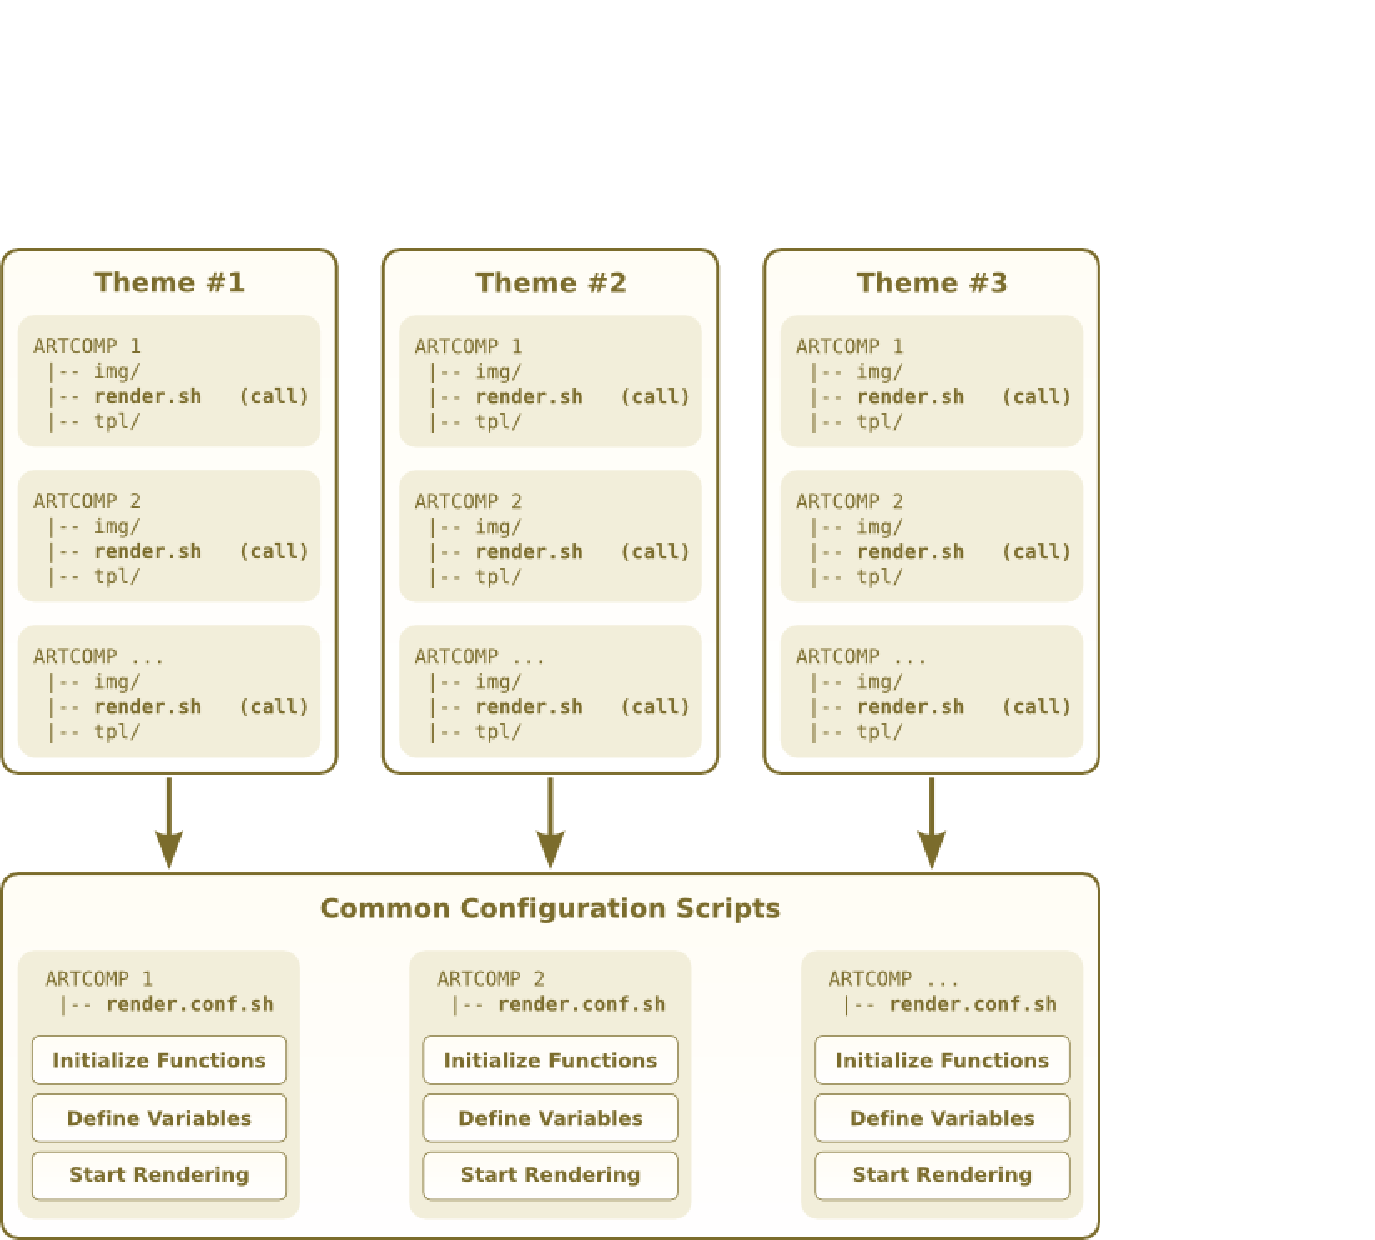
\includegraphics[width=0.8\textwidth]{%
   ../Identity/Models/Img/en/Scripts/initFunctions.pdf}
\caption{The scripts organization model.%
   \label{fig:Concepts:Scripts}}
\end{figure}

\section{Invocation Scripts}
\hypertarget{sec:Concepts:Scripts:Invocation}{}
\label{sec:Concepts:Scripts:Invocation}

Invocation scripts are identified by the name \texttt{render.sh}. You
may find invocation scripts inside \texttt{trunk/Translations/} and
\texttt{trunk/Identity/} structures.  Invocation scripts' main purpose
is calling the appropriate configuration script.

\section{Configuration Scripts}
\hypertarget{sec:Concepts:Scripts:Configuration}{}
\label{sec:Concepts:Scripts:Configuration}

\begin{description}
\item[framework:] trunk/Scripts/Config/
\end{description}

\noindent Configuration scripts are identified by the name
\texttt{render.conf.sh}. In the script organization model
(\autoref{fig:Concepts:Scripts}), configuration scripts are the first
scripts executed by you after running the invocation script
(\texttt{render.sh}).  Generally, configuration scripts are short
files that initialize functions, set variable definitions, and call
the appropriate function to start rendering.

\subsection{Initialize Functions}

Function initialization is the first action you do inside
configuration scripts.  By default, functions are initialized using
the \texttt{initFunctions.sh} script, as illustrated in
\autoref{fig:Concepts:Scripts:Configuration:initFunctions}.  The
\texttt{initFunctions.sh} script looks for functions definitions in
files that match the expansion \texttt{*.sh} inside the
\texttt{trunk/Scripts/Functions/} path, and exports them to the
current shell environment, that created when you ran the invocation
script.

\begin{figure}[!hbp]
\hrulefill
\begin{verbatim}
# Initialize functions.
. /home/centos/artwork/trunk/Scripts/initFunctions.sh
\end{verbatim}
\hrulefill
\caption{Function initialization inside configuration scripts.%
   \label{fig:Concepts:Scripts:Configuration:initFunctions}}
\end{figure}

Once functions are initialized, they are ready to be used by you, in
any point after its initialization.  This initialization arms you with
a customizable set of functionalities that can be used on
configuration scripts and reused inside functions themselves.

\subsection{Define Artwork Component}

The \texttt{ARTCOMP} variable defines the artwork component you want
to render.  The \texttt{ARTCOMP}'s value defines the specific artwork
component's matching list and Themes' translation path.  The
\texttt{ARTCOMP}'s value is built using the translation path structure
as reference.  For example, if you want to render Anaconda progress
files, you need to know that artwork component's translation path
which is:\\
\\
\fbox{trunk/Translations/Identity/Themes/Distro/Anaconda/Progress}\\
\\
and then, go to its \texttt{render.conf.sh} file to define
\texttt{ARTCOMP} as the following:\\
\\
\fbox{ARTCOMP='Distro/Anaconda/Progress'}\\
\\
The \texttt{ARTCOMP}'s value is processed by \texttt{getMatchingList}
function to determine the specific artwork component's
translation-design matching list. The matching list function is
described in \autoref{sec:Concepts:Scripts:Function:getMatchingList}.

\subsection{Define Filtering Pattern}

The \texttt{REGEX} variable defines a regular expression as filtering
pattern.  If the filtering pattern is specified, the rendering process
is limited to the amount of files matching the filtering pattern.  By
default, this value is set to receive the shell's first argument
(\texttt{\$1}).  This let you pass the filtering pattern on the
command line, at rendering time.  If you need a fixed value for the
filtering pattern, you can change the \texttt{REGEX}'s value on your
working copy to whatever you need, but please do no commit that.

\begin{figure}[!hbp]
\hrulefill
\begin{verbatim}
# Define filtering pattern. This is a regular expression 
# matching the translation path.
REGEX="$1"
\end{verbatim}
\hrulefill
\caption{Define filtering pattern inside configuration scripts.%
   \label{fig:Concepts:Scripts:Configuration:REGEX}}
\end{figure}

\subsection{Define Post-rendering Actions}
\hypertarget{sec:Concepts:Scripts:Configuration:ACTIONS}{}
\label{sec:Concepts:Scripts:Configuration:ACTIONS}

Post-rendering actions are specific functionalities applied to the
final files produced by base rendering functions like
\texttt{renderImage} and \texttt{renderText}.  Post-rendering actions
are defined by the \texttt{ACTIONS} array variable.  By default, the
\texttt{ACTIONS}'s value is set to empty (\texttt{ACTIONS[0]=''})
which provokes no post-rendering action to be applied. A different
configuration is illustrated on
\autoref{fig:Concepts:Scripts:Configuration:ACTIONS}. 

When rendering images, using \texttt{renderImage}, the only result you
get is in PNG format. This is enough most of the time. But in some
other situations, you need to produce the same image in many different
formats (i.e. xpm, pdf, tiff, xbm, etc.). These tasks are very
specific and are not included inside \texttt{renderImage} function.
Instead, the \texttt{renderFormats} function was created and used as
post-rendering action in these situations.

When rendering texts, using \texttt{renderText}, the only result you
get is in plain text format. Again, this is enough most of the time.
But in some other situations, you need to modify the final result to
provide some standardizations like: maximum line width, indentation of
first line different from second, one space between words, two after
sentences, etc. These tasks are very specific and are not included
inside \texttt{renderText} function. Instead, the \texttt{formatText}
function was created and used as post-rendering action in these
situations.

\begin{figure}[!hbp]
\hrulefill
\begin{verbatim}
# Define post-rendering actions. An empty value means that no
# post-rendering action is applied.
ACTIONS[0]='renderFormats: tif xpm pdf ppm'
ACTIONS[1]='groupByFormat: png tif xpm pdf ppm'
\end{verbatim}
\hrulefill
\caption[Define post-rendering actions.]{Define post-rendering\
actions. In this figure, post-rendering actions are used to produce\
tif, xpm, pdf, ppm, image formats (from the base PNG image format)\
and group them (PNG format included) inside directories. This is, all\
png files are stored inside a png directory, all xpm files are\
stored inside a xpm directory, and so on.%
   \label{fig:Concepts:Scripts:Configuration:ACTIONS}}
\end{figure}

\subsection{Start Rendering}

The start rendering section defines the base action to do when the
current configuration script is called. In this section what you do is
calling one of the following functions: \texttt{renderImage}
(\autoref{sec:Concepts:Scripts:Function:renderImage}), or
\texttt{renderText}
(\autoref{sec:Concepts:Scripts:Function:renderText}).

\section{Function Scripts}
\hypertarget{sec:Concepts:Scripts:Function}{}
\label{sec:Concepts:Scripts:Function}

\begin{description}
\item[framework:] trunk/Scripts/Functions/
\end{description}

\noindent Function scripts are, in fact, shell functions.  A shell
function stores a series of commands for later execution.  When the
name of a shell function is used as a simple command name, the list of
commands associated with that function name is executed.  Functions
are executed in the context of the current shell; no new process is
created to interpret them (contrast this with the execution  of a
shell script).

\subsection{renderImage}
\hypertarget{sec:Concepts:Scripts:Function:renderImage}{}
\label{sec:Concepts:Scripts:Function:renderImage}

Inside CentOS Artwork Repository, the \texttt{renderImage} function is
the heart of image production. The \texttt{renderImage} function takes
translation files and apply them to design templates, as specified in
the artwork componet's matching list that is been rendered. The final
result are PNG images based on design templates and translation files.

Additionally, the \texttt{renderImage} function accepts the following
post-rendering actions:

\begin{description}

\item[renderFormats:] The \texttt{renderFormats} function let you
produce different image formats from the base PNG image format.  The
amount of image formats you can produce with \texttt{renderFormats} is
limited to the amount of image formats that ImageMagick command line
image manipulation tool can support.

\item[groupByFormat:] The \texttt{renderByFormat} function let you
group similar image formats inside common directories.

\item[renderGrub:] The \texttt{renderGrub} function let you produce 14
colors images from the base PNG image format. The \texttt{renderGrub}
function is used to automate GRUB artwork component image production.
For this function to work, it is required to define the
\texttt{grub.ppm} palette first.

\item[renderSyslinux:] The \texttt{renderSyslinux} function let you
produce LSS16 images from the base PNG image format. The
\texttt{renderSyslinux} function is used to automate Anaconda prompt
artwork component image production.  For this function to work, it is
required to define the \texttt{syslinux.ppm} and \texttt{syslinux.hex}
palettes first.

\item[renderBrands:] The \texttt{renderBrands} function let you
produce different image formats from the base PNG image format.
Basically, it is does the same of \texttt{renderFormats}, plus two
colors grayscale, and emboss effect convertions that are not included
inside \texttt{renderFormats}.

\end{description}

\subsection{renderText}
\hypertarget{sec:Concepts:Scripts:Function:renderText}{}
\label{sec:Concepts:Scripts:Function:renderText}

The \texttt{renderText} function produce plain text files from text
plain design tempaltes and translation files. The \texttt{renderText}
standardize the text rendering process inside CentOS Artwork
Repository. Additionally, the \texttt{renderText} function accepts the
following post-rendering actions:

\begin{description}

\item[formatText:] The \texttt{formatText} function, let you format
plain text files. This function uses the GNU's \texttt{fmt} tool as
base to do all modifications.

\end{description}

\subsection{getMatchingList}
\hypertarget{sec:Concepts:Scripts:Function:getMatchingList}{}
\label{sec:Concepts:Scripts:Function:getMatchingList}

The matching list specifies the relation between design templates and
translation files that artwork components have. The
\texttt{renderImage} and \texttt{renderText} functions require this
information in order to work properly. 

Initially, the matching list was defined explicitly and independently
inside each artwork component's configuration script. Later, as many
of these components had just the same configuration stuff, the code
was reduced and unified inside \texttt{getMatchingList} function.
Inside \texttt{getMatchingList}, there is a case selection statement
where specific matching lists cases are defined, and one default
behaivour that match in thoses cases where none else does.  

The matching list code reduction changed the way you customize artwork
component's matching list.  From now on, you look inside configuration
files to be sure that \texttt{ARTCOMP} variable refers to the
appropriate artwork component, and inside \texttt{getMatchingList}
function to define its matching list.  For example, when rendering
Anaconda progress, its matching list specifies which translation files
apply which design templates. So, to change the matching list of this
artwork component, you need to edit the function
\texttt{getMatchingList} and set the appropriate relation there, in
the Anaconda progress matching list specification.

When setting artwork components' matching list, you can use any of the
following configuration available:

\begin{description}

\item[Configuration 1:] Specific translation files are applied to
specific design templates. In this configuration you have detailed
control over which translation files are applied to which design
template.

\begin{verbatim}
MATCHINGLIST="\
design-template-A.svg: translation-file-1.sed translation-file-2.sed
design-template-B.svg: translation-file-3.sed translation-file-4.sed
"
\end{verbatim}

Another way to write the previous example is: 

\begin{verbatim}
MATCHINGLIST="\
design-template-A.svg:\
   translation-file-1.sed\
   translation-file-2.sed
design-template-B.svg:\
   translation-file-3.sed\
   translation-file-4.sed
"
\end{verbatim}

In the above examples translation files 1 and 2 apply
design-template-A.svg. Likewise, translation files 3 and 4 apply
design-template-B.svg. That was a simple case, but what about if you
have hundreds of translation files to apply to specific design
templates? Lets say, translation files from 1 to 49 apply
design-template-A.svg and translation files from 50 to 99 apply
design-template-B.svg.  It would be tiresome to write down the name of
every single file in the above configuration. In these situations you
can ``generate'' the translation files as shown below: 

\begin{verbatim}
MATCHINGLIST="\
design-template-A.svg:\
   $(for NUMBER in $(sed 1 49);do
      echo -n translation-file-${NUMBER}.sed ' '
     done)
design-template-B.svg:\
   $(for NUMBER in $(sed 50 99);do
      echo -n translation-file-${NUMBER}.sed ' '
     done)
"
\end{verbatim}

Another interesting case is when you need to apply hundreds of
translation files to hundreds of design templates, in a file structure
where they both share a common bond path.  That is the
\texttt{Identity/Brands} artwork component case.  Writing down such a
matching list consumes lot of time.  So you can ``generate'' the
entire matching list like the following:

\begin{verbatim}
MATCHINGLIST="\
$(for TEMPLATE in $(find $(getPath 'trunk/Identity/Brands')/tpl \
   -name '*.svg' | sed -r 's!.*/Brands/Tpl/(.*)$!\1!' | sort );do

   TRANSLATION=$(find $(getPath \
      'trunk/Translations/Identity/Brands')/$(echo $TEMPLATE \
      | sed 's!\.svg!!') -name '*.sed' \
      | sed -r 's!^.*/Brands/(.*)$!\1!' \
      | sort | tr '\n' ' ')

   echo $TEMPLATE: $TRANSLATION
   done)
"
\end{verbatim}

\item[Configuration 2:] All translation files are applied to a single
design template.  In this configuration all artwork component's
translation files are applied to one design template
(design-template-A.svg for the matter of this case).

\begin{verbatim}
MATCHINGLIST="design-template-A.svg"
\end{verbatim}

\item[Configuration 3:] Translation files are applied to design
templates that share a common name. In this configuration translation
files are applied to design templates taking the name part, without
extension, as reference.  This means that, if you have a translation
file named \texttt{File-1.sed} you need to have a \texttt{File-1.svg}
inside design templates. This way, \texttt{File-1.sed} can be applied
to \texttt{File-1.svg} and, as result, produce the \texttt{File-1.png}
file.  This is the default matching list behaivour.

\begin{verbatim}
MATCHINGLIST=""
\end{verbatim}

\end{description}

\subsection{getPath}

The \texttt{getPath} function creates the artwork component's absolute
path. Before output the absolute path, \texttt{getPath} removes any
``strange'' character from the final path. For \texttt{getPath} to
work, the relative path to the artwork component should be provided
from \texttt{trunk/}'s directory level on.
